% THIS IS SIGPROC-SP.TEX - VERSION 3.1
% WORKS WITH V3.2SP OF ACM_PROC_ARTICLE-SP.CLS
% APRIL 2009
%
% It is an example file showing how to use the 'acm_proc_article-sp.cls' V3.2SP
% LaTeX2e document class file for Conference Proceedings submissions.
% ----------------------------------------------------------------------------------------------------------------
% This .tex file (and associated .cls V3.2SP) *DOES NOT* produce:
%       1) The Permission Statement
%       2) The Conference (location) Info information
%       3) The Copyright Line with ACM data
%       4) Page numbering
% ---------------------------------------------------------------------------------------------------------------
% It is an example which *does* use the .bib file (from which the .bbl file
% is produced).
% REMEMBER HOWEVER: After having produced the .bbl file,
% and prior to final submission,
% you need to 'insert'  your .bbl file into your source .tex file so as to provide
% ONE 'self-contained' source file.
%
% Questions regarding SIGS should be sent to
% Adrienne Griscti ---> griscti@acm.org
%
% Questions/suggestions regarding the guidelines, .tex and .cls files, etc. to
% Gerald Murray ---> murray@hq.acm.org
%
% For tracking purposes - this is V3.1SP - APRIL 2009

\documentclass{edm_template}

\begin{document}

\title{YouEDU: Addressing Confusion in MOOC Discussion Forums by Recommending Instructional Video Clips}
%\subtitle{[Extended Abstract]
%\titlenote{A full version of this paper is available as
%\textit{Author's Guide to Preparing ACM SIG Proceedings Using
%\LaTeX$2_\epsilon$\ and BibTeX} at
%\texttt{www.acm.org/eaddress.htm}}}
%
% You need the command \numberofauthors to handle the 'placement
% and alignment' of the authors beneath the title.
%
% For aesthetic reasons, we recommend 'three authors at a time'
% i.e. three 'name/affiliation blocks' be placed beneath the title.
%
% NOTE: You are NOT restricted in how many 'rows' of
% "name/affiliations" may appear. We just ask that you restrict
% the number of 'columns' to three.
%
% Because of the available 'opening page real-estate'
% we ask you to refrain from putting more than six authors
% (two rows with three columns) beneath the article title.
% More than six makes the first-page appear very cluttered indeed.
%
% Use the \alignauthor commands to handle the names
% and affiliations for an 'aesthetic maximum' of six authors.
% Add names, affiliations, addresses for
% the seventh etc. author(s) as the argument for the
% \additionalauthors command.
% These 'additional authors' will be output/set for you
% without further effort on your part as the last section in
% the body of your article BEFORE References or any Appendices.

\numberofauthors{3} %  in this sample file, there are a *total*
% of EIGHT authors. SIX appear on the 'first-page' (for formatting
% reasons) and the remaining two appear in the \additionalauthors section.
%
\author{
% You can go ahead and credit any number of authors here,
% e.g. one 'row of three' or two rows (consisting of one row of three
% and a second row of one, two or three).
%
% The command \alignauthor (no curly braces needed) should
% precede each author name, affiliation/snail-mail address and
% e-mail address. Additionally, tag each line of
% affiliation/address with \affaddr, and tag the
% e-mail address with \email.
%
% 1st. author
\alignauthor Akshay Agrawal\\
       \affaddr{Stanford University}\\
       \email{akshayka@cs.stanford.edu}
% 2nd. author
\alignauthor Jagadish Venkatraman\\
       \affaddr{Stanford University}\\
       \email{vjagadish@cs.stanford.edu}
% 3rd. author
\alignauthor Andreas Paepcke\\
       \affaddr{Stanford University}\\
       \email{paepcke@cs.stanford.edu}
% \and   use '\and' if you need 'another row' of author names
}
\date{9 February 2015}
% Just remember to make sure that the TOTAL number of authors
% is the number that will appear on the first page PLUS the
% number that will appear in the \additionalauthors section.

\maketitle
\begin{abstract}
In Massive Open Online Courses (MOOCs), struggling learners often seek help by
posting questions in discussion forums. Unfortunately, given the large volume of discussion in MOOCs, instructors may overlook these learners' posts,
detrimentally impacting the learning process and exacerbating attrition. In this paper, we present YouEDU, an instructional aid that automatically detects and addresses confusion in forum posts. Leveraging our publicly-available Stanford MOOCPosts corpus, we train a heterogeneous set of classifiers to classify forum posts across multiple dimensions. In particular, classifiers that target sentiment, urgency, and other descriptive variables inform a single classifier that detects confusion. We then employ information retrieval techniques to map confused posts to minute-resolution clips from course videos; the ranking over these clips accounts for both video-clickstream data and textual similarity between posts and closed captions. We measure the performance of our classification model in multiple educational contexts, exploring the nature of confusion within each; we also evaluate the relevancy of materials returned by our ranking algorithm.
\end{abstract}

%% A category with the (minimum) three required fields
%\category{H.4}{Information Systems Applications}{Miscellaneous}
%%A category including the fourth, optional field follows...
%\category{D.2.8}{Software Engineering}{Metrics}[complexity measures, performance measures]
%
%\terms{Theory}

\keywords{ACM proceedings, \LaTeX, text tagging} % NOT required for Proceedings

\section{Introduction}
* Proliferation of MOOCs\\
* Volume of posts high\\
* Difficult to get a birds-eye view of the course, difficult to address it.\\

* Work looking into sentiment thus far is limited by datasets\\
* Work has been done on confusion, but not so much on MOOCs (save Rosé)\\
* Work into intelligently intervening + aiding the instructor\\
* Previous work has found forum to perhaps not be the most useful, even\\
* We suspect that the forum's perceived lack of usefulness is not instrinsic but rather ~ lack of attention lack of instructor tools + isolation from other parts of the classroom.\\
* We accordingly set out to adress both of these problems -- mining for affect gives instructors a pulse on the state of the course, and linking to videos marries forum and other course resources.\\
* Why video snippets as opposed to videos? \cite{Guo:2014:VPA:2556325.2566239} -- in a retrospective study of four edX courses, the maximum median engagement, regardless of video length, was six minutes.

The remainder of this paper is organized as follows. We examine related work in section two, present the Stanford MOOCPosts corpus in section three, sketch the architecture of YouEDU in section four, detail YouEDU's constituent classification and recommendation phases, evaluating both and interpreting results in sections five and six, and propose future work in section seven.

\section{Related Work}

\section{The Stanford MOOCPosts Corpus}
A precondition to automatically detecting affect in MOOC discussion forums was manually identifying it; given that no publicly-available corpus of tagged MOOC discussion forum posts existed prior to our research, we set out to create our own. The outcome of our data compilation and curation was the Stanford MOOCPosts dataset: a corpus composed of 29,604 anonymized learner forum posts from eleven Stanford University public online classes. Freely available to academic researchers, the MOOCPosts dataset was designed to enable computational inquiries into the nature of both affect and content in MOOC discussion forums.

Each post in the MOOCPosts dataset was scored across six dimensions -- confusion, sentiment, urgency, question, answer, and opinion -- and subsequently augmented with additional metadata. In this section, we detail the data collection methodology, defining each of the six dimensions along the way, and briefly present some insights gleaned by mining the set.


\subsection{Methodology: Compiling the Dataset}
Nine judges from oDesk were hired to ...

\subsection{Insights and Discussion}
We report insights gleaned into the nature of affect, etc. across these courses.

% TODO: Is this really the right place to present this? Or should this
% be presented in the Classification Combination Section?
\subsubsection{Relationship between Variables}
In this section, we report the pairwise correlations between variables to 1) shed some light into the nature of each and also 2) to motivate a YouEDU design choice.

% TODO: Perhaps fold this into the introduction.
\section{YouEDU: Detect and Recommend}

%TODO: Display + Caption
YouEDU is a personalized intervention system that recommends educational video clips to learners. Figure \ref{figure:architecture} illustrates the key steps that comprise YouEDU. YouEDU takes as input a set $P$ of forum posts, processing them in two distinct phases: (I) detection and (II) recommendation. In the first phase, we apply a classifier to each post in $P$, outputting a subset $P_{c}$ consisting of posts in which the classifier detected confusion. The confusion classifier functions as a \emph{combination} classifier in that it combines the predictions from classifiers trained to predict other post-related qualities.

\begin{figure}[ht]
       \centering
       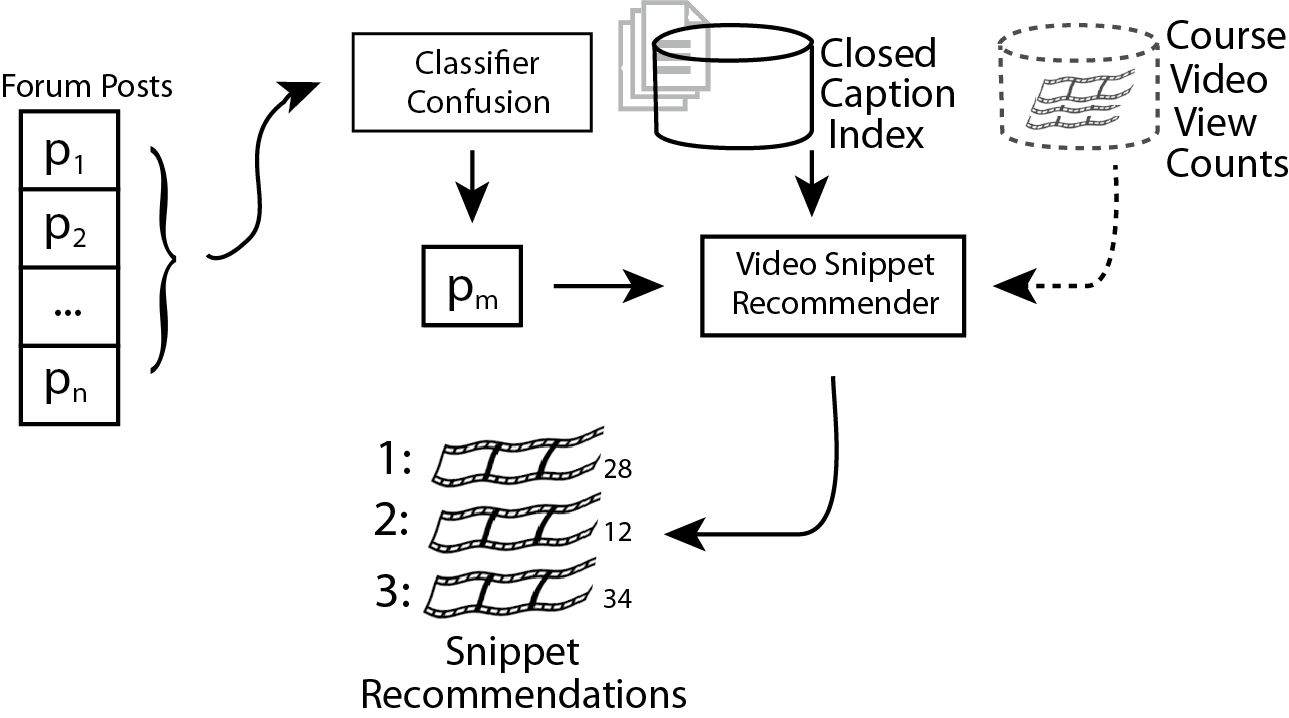
\includegraphics[width=0.5\textwidth]{../Figs/youEduArch.png}
       \caption{\textnormal{YouEDU Architecture. The YouEDU pipeline consists of two phases: post classification and video snippet recommendation.}}
       \label{figure:architecture}
\end{figure}

The second phase takes $P_{c}$ as input and, for each confused post in $p \in P_{c}$, outputs a ranked list of educational video snippets that address the object of confusion expressed in $p$. In particular, for a given post, the recommender produces an initial ranking across a number of one-minute video clips by computing a similarity metric between the post and closed caption sections. The ranking of videos in the retrieved set is then further informed by video-clickstream data.

While YouEDU outputs minute-resolution video clips, it does not necessarily guarantee that these clips fully address the exhibited confusion -- indeed, several minutes of instructional content are often required to explain a single concept. Rather, the video snippets collectively form an ad-hoc index. For example, say that for a given post, YouEDU outputs three video snippets with start times $s_{1}, s_{2}, s_{3}$, in order of decreasing relevance, and say that these snippets were contained in videos $v_{1}, v_{2}, v_{3}$, respectively, $v_{1}, v_{2}, v_{3}$ not necessarily unique. In order to clarify his or her confusion, the author of the post should begin watching video $v_{1}$ at $s_{1}$ -- the learner can autonomously set the end time of the snippet, and can move on to the next video, start time pair if any confusion still lingers. 

In the following two sections, we delve further into both phases of YouEDU, describing them in detail and relating the results of empirical evaluations.

\section{Phase I: Detecting Confusion}
In this section, we present the model used to classify confusion. At a high-level, we use a coordinated combination of classifiers ...

\subsection{Classifier Design}
\subsubsection{Feature Space}
Here's an intuition of what we figured might be helpful across all variables ...

* Bag of Words \\
(* Specific Bigrams / words / trigrams? Time permitting) \\
* Pre-processing Steps \\
* Features Extracted / Generated \\

\subsubsection{A Combination of Hypotheses}
* Classifier Combination -- Overview \\
* Our particular implementation \\
* Subclassifiers ~ Variable-Specific Features \\
* Training, use gold values, testing, use predicted values \\
* Combination Step ~ Logistic Regression Layer \\

\subsection{Evaluation}

* educational contexts \\
* metrics used \\ 
* results \\
* implications \\

\section{Phase II: Recommending Clips}
\subsection{The Recommendation Algorithm}
\subsubsection{Retrieval}
\subsubsection{Ranking}

\subsection{Evaluation}
Two experts were hired ...

\section{Future Work}
Future work might focus on strengthening the link between the classifiers and the reccomendation system; in particular, it would behoove us to devise a way to filter our set of confused posts to a subset for which recommendation makes sense. Additionally, we might want to make our classifiers better and index back into the previous course to retrieve answers for courses. Deploying this system live is another thing that we might do. 

YouEDU's two phases need not be packaged together; in an online setting, they could operate as independent, complemetary services. The output of Phase I could be presented directly to instructors, many of whom express interest in understanding activity in discussion forums \cite{Stephens-Martinez:2014:MMI:2556325.2566246}. As for Phase II, the recommendation system might live as a search-box of sorts: learner would type natural language queries in which they voiced their confusion, and our system would serve them relevant resources.

\section{Conclusion}
YouEDU takes an initial step towards building automated confusion intervention ... 

%\end{document}  % This is where a 'short' article might terminate

%ACKNOWLEDGMENTS are optional
\section{Acknowledgments}
This section is optional\cite{wen2014sentiment}; it is a location for you
to acknowledge grants, funding, editing assistance and
what have you.  In the present case, for example, the
authors would like to thank Gerald Murray of ACM for
his help in codifying this \textit{Author's Guide}
and the \textbf{.cls} and \textbf{.tex} files that it describes.

%
% The following two commands are all you need in the
% initial runs of your .tex file to
% produce the bibliography for the citations in your paper.
\bibliographystyle{abbrv}
\bibliography{sources}  % sigproc.bib is the name of the Bibliography in this case
% You must have a proper ".bib" file
%  and remember to run:
% latex bibtex latex latex
% to resolve all references
%
% ACM needs 'a single self-contained file'!
%
%APPENDICES are optional
%\balancecolumns
\balancecolumns
% That's all folks!
\end{document}
